\documentclass[11pt,a4paper]{amsart}
\usepackage[utf8]{inputenc}
\usepackage[T1]{fontenc}
\usepackage{lmodern}
\usepackage{amsmath,amssymb,amsthm}
\usepackage{booktabs}
\usepackage{graphicx}
\usepackage[margin=2.3cm]{geometry}
\usepackage{xcolor}
\usepackage[colorlinks=true,linkcolor=blue!50!black,citecolor=blue!50!black,urlcolor=blue!50!black]{hyperref}

\newtheorem{theorem}{Theorem}
\newtheorem{lemma}[theorem]{Lemma}
\newtheorem{proposition}[theorem]{Proposition}
\newtheorem{corollary}[theorem]{Corollary}
\theoremstyle{remark}
\newtheorem*{remark}{Remark}

\newcommand{\dd}{\,\mathrm{d}}
\newcommand{\tp}{t'}

\title[Variational and exponential-sum estimates in Granville's survey]{A note on the variational and exponential-sum estimates in Granville's \texorpdfstring{\lq\lq Primes in intervals of bounded length\rq\rq}{"Primes in intervals of bounded length"}}
\thanks{Code and data are archived at Zenodo, \href{https://doi.org/10.5281/zenodo.24296047}{doi:10.5281/zenodo.24296047};\\ repository: \href{https://github.com/Ruqing1963/granville-2015-bams-audit}{github.com/Ruqing1963/granville-2015-bams-audit}.}
\author{Ruqing Chen}
\address{GUT Geoservice Inc., Montreal, Canada}
\email{ruqing@hotmail.com}
\date{November 16, 2026}
\subjclass[2020]{11N05, 11N36, 11L05}
\keywords{bounded gaps between primes, Maynard--Tao sieve, variational problem, Graham--Ringrose method}

\begin{document}
\begin{abstract}
We revisit the self-contained lower bound for Maynard's ratio $\rho(F)$ in Sections~6.8--6.9 of
A.~Granville's survey \emph{Primes in intervals of bounded length} (Bull.\ Amer.\ Math.\ Soc.\ \textbf{52}
(2015), 171--222). (i) The survey rewrites the numerator of $\rho(F)$ as $L_k-M_k$. In fact
$k\int(A-B)^2\le L_k-kM_k$, with strict inequality, so this is an \emph{upper} bound, whereas the
argument needs a lower bound. Moreover, the factor $k$ is missing from the definition of $M_k$.
(ii) The parameter $\eta$ in Section~6.9 should be $(1-(A+1)e^{-A})/(A(1-e^{-A}))$, not
$(1-(A-1)e^{-A})/(A(1-e^{-A}))$. The final inequality in (6.8) is nevertheless correct, because
$(1-(A+1)x)^2-(1-x)^2(1-2Ax-x^2)=x^2(A-1+x)^2$. (iii) We give two rigorous repairs. Young's inequality
gives $\rho(F)\ge\frac12\log k-2$, which proves Theorem~6.4 under $k>e^{8m+4}$ in place of
$k\log k>e^{8m+4}$. Truncating the support in $k-1$ variables gives
$\rho(F)\ge\log k-2\log\log k-\frac12$ for $k\ge e^{7}$. This recovers Theorem~6.4 and Corollary~6.5
exactly as stated. (iv) In Part~2 we correct a Fourier cutoff in Section~9.3 and two misprints, and we
resolve a notational ambiguity in Section~11.2. Two further passages that look like slips are correct as
printed.
\end{abstract}
\maketitle

\section{Introduction}

Granville's survey \cite{G} explains Zhang's \cite{Z} and Maynard's \cite{M} theorems (see also \cite{P}) on bounded gaps
between primes. Its Section~6 contains a short self-contained proof that the Maynard ratio
\[
\rho(F)=\frac{k\int_{t_1,\dots,t_{k-1}\ge0}\bigl(\int_{t_k\ge0}F\dd t_k\bigr)^2\dd t_{k-1}\cdots\dd t_1}
{\int_{t_1,\dots,t_k\ge0}F^2\dd t_k\cdots\dd t_1}
\]
can be made larger than $4m$. This leads to Theorem~6.4 (if $k\log k>e^{8m+4}$, then any admissible
$k$-tuple has at least $m$ prime values infinitely often) and to Corollary~6.5 ($B_m=e^{8m+5}$).

We check this argument line by line and find one genuine gap: an inequality is used in the wrong
direction (Section~\ref{sec:68}). The other slips in Sections~6.8--6.9 turn out to be harmless
(Section~\ref{sec:69}). In Section~\ref{sec:repair} we close the gap in two ways. The first keeps
Granville's variance method and absorbs the cross term by Young's inequality. The second avoids the cross
term by truncating the support, and it recovers Theorem~6.4 and Corollary~6.5 without change.
Section~\ref{sec:part2} collects remarks on the exposition of Zhang's theorem in Part~2.

All page numbers refer to \cite{G}. The identities were verified symbolically, and the numbers were
checked independently in two ways. First, we computed $\rho(F)$ exactly, up to discretisation, by FFT
convolution of the relevant probability law. Second, we evaluated the Young and Chebyshev bounds
directly. The program is provided as supplementary material.

\section{The numerator of \texorpdfstring{$\rho(F)$}{rho(F)} in Section~6.8}\label{sec:68}

Section~6.8 (p.~200) takes $F(t_1,\dots,t_k)=g(kt_1)\cdots g(kt_k)$ on $t_1+\dots+t_k\le1$ and $F=0$
otherwise, with $g\ge0$ supported on $[0,T]$, $\gamma=\int g^2$ and $\mu=\int tg(t)^2\dd t$. For
$\tp=(t_1,\dots,t_{k-1})$ write $s=t_1+\dots+t_{k-1}$ and
\[
A(\tp)=\int_{t_k\ge0}\prod_{i\le k}g(kt_i)\dd t_k,\qquad
B(\tp)=\int_{t_k\ge\max(0,1-s)}\prod_{i\le k}g(kt_i)\dd t_k .
\]
Then $\int_{t_k\ge0}F\dd t_k=A-B$ with $0\le B\le A$, so the numerator of $\rho(F)$ is
\begin{equation}\label{eq:N}
N_k=k\int_{\tp\ge0}\bigl(A(\tp)-B(\tp)\bigr)^2\dd\tp .
\end{equation}

\subsection*{The reversal}
The paper says \lq\lq We rewrite the numerator of $\rho(F)$ as $L_k-M_k$\rq\rq, with
$L_k=k\int A^2$ and $M_k=\int B^2$ (p.~200). Since $(A-B)^2-(A^2-B^2)=-2B(A-B)\le0$,
\begin{equation}\label{eq:rev}
N_k=L_k-k\int_{\tp\ge0}\bigl(2AB-B^2\bigr)\dd\tp\ \le\ L_k-kM_k ,
\end{equation}
and the inequality is strict as soon as $0<B<A$ on a set of positive measure. This always happens: if
$T>1$ (equivalently $A>0$ in Section~6.9) then $B$ vanishes for $s\le1-T/k$ and equals $A$ for $s\ge1$,
and $0<B<A$ in between. Thus $L_k-kM_k$ is an upper bound for the numerator, but inequality (6.7)
treats it as a lower bound. Closing the gap requires a bound for the cross term $2AB$. In $AB$ the tail
integral $\int_{t_k\ge1-s}g(kt_k)\dd t_k$ appears only to the first power. The Cauchy--Schwarz step on
p.~200 bounds the \emph{square} of this integral by $(T/k)\int_{t_k\ge1-s}g(kt_k)^2\dd t_k$, and so it
does not apply to $AB$ as it stands. Table~\ref{tab:num} and the inset of Figure~\ref{fig:main}(a) show that
the gap in \eqref{eq:rev} is large for small $k$.

\subsection*{The missing factor \texorpdfstring{$k$}{k}}
The display defining $M_k$ has no factor $k$, although $L_k$ does. Under that literal definition the
Cauchy--Schwarz step over an interval of length $\le T/k$, followed by $u_j=kt_j$, gives
$M_k\le k^{-k-1}T\int_{u_1+\dots+u_k\ge k}\prod g(u_i)^2\dd u$. The printed bound has $k^{-k}T$, which is
the bound for $kM_k$. So the intended object is $kM_k=k\int B^2$, as in \eqref{eq:rev}.

\begin{remark}\label{rem:var}
The penultimate display on p.~200 replaces $\bigl(\tfrac1k(u_1+\dots+u_k)-\mu/\gamma\bigr)^2$ by
$k^{-1}(u_1^2-\mu^2/\gamma^2)$ under $\int\prod g(u_i)^2$. This may look like a misprint for
$(u_1-\mu/\gamma)^2$, but it is \emph{correct as printed}. The two integrals coincide because
$\int g(u)^2(u-\mu/\gamma)^2\dd u=\int u^2g^2-\mu^2/\gamma=\int g(u)^2(u^2-\mu^2/\gamma^2)\dd u$. The
variance bound $kM_k\le\eta^{-2}k^{-k-1}T\gamma^{k-1}\int u^2g(u)^2\dd u$ is therefore valid when
$\mu\le(1-\eta)\gamma$.
\end{remark}

\section{The parameter \texorpdfstring{$\eta$}{eta} and inequality (6.8)}\label{sec:69}

For $g(t)=1/(1+At)$ on $[0,T]$ with $1+AT=e^A$, the values on p.~201 are correct:
$\gamma=(1-e^{-A})/A$, $\mu=(A-1+e^{-A})/A^2$, $\int t^2g^2=(e^A-2A-e^{-A})/A^3$ and $\int g=1$. However,
\[
\eta=1-\frac{\mu}{\gamma}=\frac{1-(A+1)e^{-A}}{A(1-e^{-A})},\qquad\text{whereas p.~201 prints}\qquad
\frac{1-(A-1)e^{-A}}{A(1-e^{-A})}.
\]
The printed value exceeds the true one by $2/(A(e^A-1))$ (Figure~\ref{fig:main}(b), inset). Write
$x=e^{-A}$ and use $T=(e^A-1)/A=e^A(1-x)/A$. With the correct $\eta$, the middle expression of (6.8) is
\begin{equation}\label{eq:68}
\frac{A}{1-x}-\frac{e^{2A}}{Ak}\,R(A),\qquad
R(A)=\frac{(1-2Ax-x^2)(1-x)^2}{(1-(A+1)x)^2},
\end{equation}
so the slip $A-1\mapsto A+1$ changes only the denominator. The final step of (6.8), namely
$\ge A-e^{2A}/(Ak)$, still holds for every $A>0$ and $k\ge1$. It does not even need to borrow from
$A/(1-x)-A=Ax/(1-x)$, because of the polynomial identity
\begin{equation}\label{eq:R}
(1-(A+1)x)^2-(1-x)^2(1-2Ax-x^2)=x^2(A-1+x)^2\ \ge0,
\end{equation}
which gives $R(A)\le1$. With the printed $\eta$ the denominator is even larger, so the printed middle
term is smaller than the true one, and the final bound in (6.8) is unaffected. Hence, once the gap of
Section~\ref{sec:68} is closed, the only effect of the misprint is cosmetic.

\section{Two rigorous repairs}\label{sec:repair}

From now on $g(t)=1/(1+At)$ on $[0,T]$ with $A>1$, and $\ell=\log k$. The denominator of $\rho(F)$ is at
most $k^{-k}\gamma^k$, as on p.~200, and $L_k=k^{-k}\gamma^{k-1}$. Moreover
$1/\gamma=A/(1-e^{-A})\ge A$.

\begin{proposition}[Young's inequality]\label{prop:young}
For every $\theta\in(0,1)$, $\rho(F)\ge(1-\theta)\bigl(A-e^{2A}/(\theta Ak)\bigr)$. Consequently, if
$e^A<A\sqrt k$, then $\rho(F)\ge A\bigl(1-e^A/(A\sqrt k)\bigr)^2$. In particular, for $k>e^2$,
\[
\rho(F)\ \ge\ \tfrac12\log k-2+\tfrac{2}{\log k}\qquad(A=\tfrac12\log k).
\]
\end{proposition}

\begin{proof}
We have $(a-b)^2-(1-\theta)(a^2-\theta^{-1}b^2)=(\sqrt\theta\,a-b/\sqrt\theta)^2\ge0$, so
$N_k\ge(1-\theta)(L_k-\theta^{-1}kM_k)$. Now $B^2$ enters squared and with a minus sign. Hence the
Cauchy--Schwarz and variance bounds of p.~200 (with the factor $k$ of Section~\ref{sec:68} and
the Remark in Section~\ref{sec:68}) apply verbatim. Dividing by $k^{-k}\gamma^k$ and using \eqref{eq:68}--\eqref{eq:R}
gives $\rho(F)\ge(1-\theta)(a-b/\theta)$ with $a=1/\gamma\ge A$ and $b\le e^{2A}/(Ak)$. Maximising over
$\theta$ (at $\theta=\sqrt{b/a}$) gives $(\sqrt a-\sqrt b)^2\ge A(1-e^A/(A\sqrt k))^2$. For $A=\ell/2$
this equals $\frac{\ell}2(1-\frac2\ell)^2$.
\end{proof}

Proposition~\ref{prop:young} gives $\rho(F)>4m$ once $\log k\ge8m+4$. This proves Theorem~6.4 with
\lq\lq$k\log k>e^{8m+4}$\rq\rq\ replaced by \lq\lq$k>e^{8m+4}$\rq\rq. The prime-counting argument on
p.~202 then gives Corollary~6.5 with $B_m=(16m+9)e^{8m+4}$ instead of $e^{8m+5}$. Proposition~\ref{prop:young}
is not enough for the statement as printed. The optimised Young bound at the least $k$ with
$k\log k>e^{8m+4}$ falls short of $4m$ for every $m\le60$ that we tested (e.g.\ $3.29$ against $4$ for
$m=1$). The reason is that it loses the term $\frac12\log\log k$ claimed in (6.8).

\begin{proposition}[Truncation in $k-1$ variables]\label{prop:trunc}
Let $k\ge e^{7}$ and $A=\log k-2\log\log k$. Then
\[
\rho(F)\ \ge\ \log k-2\log\log k-\tfrac12 .
\]
\end{proposition}

\begin{proof}
The idea is to keep only the region where the tail $B$ vanishes identically. There the integrand of
\eqref{eq:N} is exactly $A^2$, so neither the cross term $2AB$ nor the Cauchy--Schwarz bound for $B^2$
is needed. Precisely, if $s\le1-T/k$, then $g(kt_k)=0$ for $t_k\ge1-s$, so $B(\tp)=0$ and $(A-B)^2=A^2$. Discarding the rest of
\eqref{eq:N} and putting $u_i=kt_i$, we get
\[
N_k\ge k\int_{s\le1-T/k}A(\tp)^2\dd\tp=k^{-k}\gamma^{k-1}\bigl(1-\Pr[S_{k-1}>k-T]\bigr).
\]
Here $S_{k-1}$ is a sum of $k-1$ independent variables with density $g^2/\gamma$ on $[0,T]$. Their mean is
$1-\eta$ and their variance is $v\le\int u^2g^2/\gamma\le e^A/(A^2(1-e^{-A}))$. In particular,
the factor $T\approx e^A/A$ lost in the Cauchy--Schwarz step does not appear. By Chebyshev's inequality,
\[
\Pr[S_{k-1}>k-T]\le P:=\frac{(k-1)v}{\bigl((k-1)\eta+1-T\bigr)^2}.
\] For $\ell\ge7$ we have $A\ge3.1$, so
$\eta\ge(1-4e^{-3})/A\ge0.8/A$ and $T\le e^A/A=k/(A\ell^2)$. Hence $(k-1)\eta+1-T\ge(0.8-\ell^{-2})k/A\ge0.77\,k/A$
and $P\le e^A/(0.56\,k)=1/(0.56\,\ell^2)$. Therefore
$\rho(F)\ge A(1-P)\ge A-1/(0.56\,\ell)\ge\ell-2\log\ell-0.26$.
\end{proof}

\begin{corollary}\label{cor:64}
Theorem~6.4 holds as stated for every $m\ge1$, and Corollary~6.5 holds with $B_m=e^{8m+5}$ for $m\ge2$.
\end{corollary}

\begin{proof}
Let $k$ be least with $k\log k>e^{8m+4}$, and let $\ell=\log k$. Then $\ell\ge9.72$, $\ell+\log\ell>8m+4$ and
$\ell<8m+4$. Proposition~\ref{prop:trunc} gives
$\rho(F)\ge\ell-2\log\ell-\frac12>8m+\frac72-3\log(8m+4)$, and this exceeds $4m$ for all $m\ge1$ (the
difference increases in $m$ and equals $0.045$ at $m=1$). The remaining steps of Section~6.9 do not use
the shape of $F$.
\end{proof}

Proposition~\ref{prop:trunc} has the same leading term $\log k$ as Maynard's bound (6.9). Numerically,
the exact value of $\rho(F)$ at Granville's choice $A=\frac12(\ell+\log\ell)$ is computed by FFT
convolution of the law of $S_{k-1}$ (Table~\ref{tab:num}). It stays above the bound claimed in (6.8) for
$5\le k\le1000$. So the gap affects only the proof, and the conclusion is true.

\begin{table}[ht]
\centering\small
\caption{Left: $N_k/L_k$ against $(L_k-kM_k)/L_k$ for $A=2$. Right: exact $\rho(F)$ at
$A=\frac12(\log k+\log\log k)$, compared with the bound claimed in (6.8) and Tao's upper bound
$k\log k/(k-1)$.}\label{tab:num}
\begin{tabular}{rcc@{\qquad}rccc}
\toprule
$k$ & $N_k/L_k$ & $(L_k-kM_k)/L_k$ & $k$ & $\rho(F)$ & claim (6.8) & Tao \\
\midrule
2  & 0.4397 & 0.8012 & 10   & 1.9216 & $-0.4317$ & 2.5584\\
5  & 0.6998 & 0.8672 & 50   & 2.8103 & 0.6380 & 3.9919\\
10 & 0.8567 & 0.9301 & 200  & 3.5849 & 1.4829 & 5.3249\\
20 & 0.9584 & 0.9784 & 500  & 4.0922 & 2.0208 & 6.2271\\
50 & 0.9984 & 0.9991 & 1000 & 4.4736 & 2.4202 & 6.9147\\
\bottomrule
\end{tabular}
\end{table}

\begin{figure}[ht]
\centering
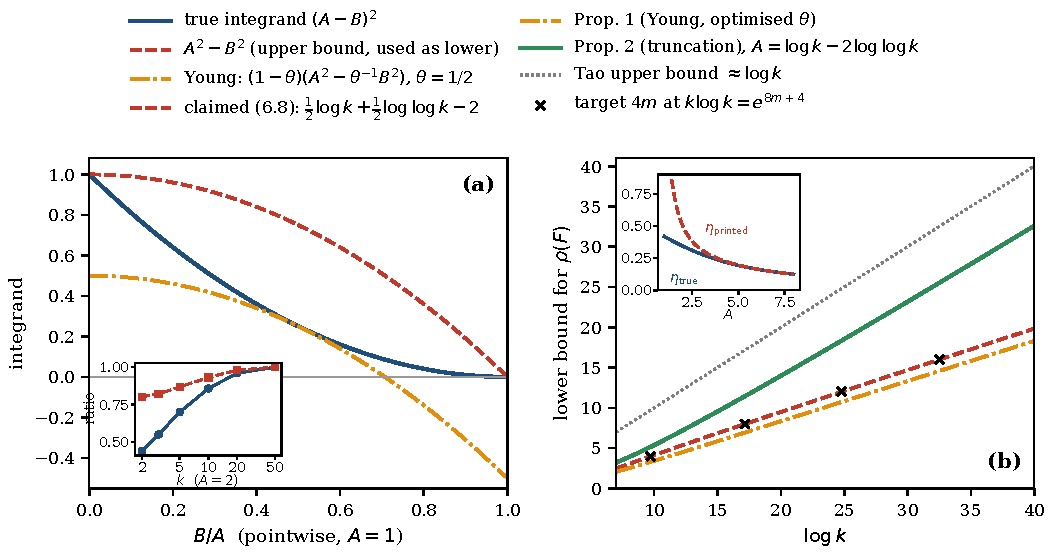
\includegraphics[width=\textwidth]{figures/fig_granville_2015_audit.pdf}
\caption{(a) Pointwise integrands as functions of $B/A$. The inset shows the integrated ratios $N_k/L_k$
(blue) and $(L_k-kM_k)/L_k$ (red) for $A=2$. (b) Lower bounds for $\rho(F)$ against $\log k$, with the
targets $4m$ at the least $k$ satisfying $k\log k>e^{8m+4}$ ($m=1,\dots,4$). The inset compares
$\eta_{\rm true}$ and $\eta_{\rm printed}$ as functions of $A$.}\label{fig:main}
\end{figure}

\section{Remarks on Part 2}\label{sec:part2}

\emph{Section 9.3 (p.~211).} In (9.4), for a progression modulo $q$ in an interval of length $M$, the
cutoffs are $H_j=2^jq/M$. In the next two displays the inner progression has modulus
$rg\ell_1\ell_2\asymp RQ^2/g$, since $\ell_i\asymp Q/g$. The third display, however, sets $H_j:=2^jG/g$.
Here $G$, which appears only as the range $g\le G$, is never defined, and the quantity is not of the form
$2^j\cdot(\text{modulus})/M$. It should read $H_j:=2^jrg\ell_1\ell_2/M\asymp2^jRQ^2/(gM)$.

\emph{Section 11.2 (pp.~214--215).} The identity
$e_q(f(n+kq_1))=e_{q_1}(f(n)/q_2)\,e_{q_2}(f(n+kq_1)/q_1)$ is false if \lq\lq$/q_2$\rq\rq\ means real
division, which is how $e_m(t)=e(t/m)$ is defined on p.~210. In that case the right side equals
$e_q(f(n))e_q(f(n+kq_1))$. Our test with random coprime $q_1,q_2$ and integer arguments found the
identity false in $1986$ of $2000$ cases. The paper elsewhere uses \lq\lq$/$\rq\rq\ inside $e_q(\cdot)$
for division modulo the modulus ($C_1/n$ in (10.2), and \lq\lq$(\mathrm{mod}\ q_2)$\rq\rq\ in $g_{k,k'}$). Under
that reading the identity is correct for squarefree $q=q_1q_2$:
\[
e_q(f(n+kq_1))=e_{q_1}\bigl(\overline{q_2}\,f(n+kq_1)\bigr)\,e_{q_2}\bigl(\overline{q_1}\,f(n+kq_1)\bigr)
=e_{q_1}\bigl(\overline{q_2}\,f(n)\bigr)\,e_{q_2}\bigl(\overline{q_1}\,f(n+kq_1)\bigr),
\]
with $\overline{q_2}q_2\equiv1\pmod{q_1}$ and $\overline{q_1}q_1\equiv1\pmod{q_2}$. The second
equality uses $f(n+kq_1)\equiv f(n)\pmod{q_1}$, which needs $\overline{q_2}\in\mathbb Z$. This
matches the device $e_{rs}(m)=e_s(am)e_r(bm)$ of Section~10.2. Writing $\overline{q_2},\overline{q_1}$
explicitly removes the ambiguity. The argument itself is not affected.

\emph{Misprints.} On p.~197, $T_k$ is defined with \lq\lq each $t_j\ge1$\rq\rq; this should be $t_j\ge0$
(otherwise $T_k=\emptyset$ for $k\ge2$). On p.~207, the upper comparison sum
$\sum_{n_+\le n\le n_+-1}\log qn$ is empty. It should be $\sum_{n_-+1\le n\le n_+}\log qn$.

\begin{thebibliography}{9}
\bibitem{G} A.~Granville, \emph{Primes in intervals of bounded length}, Bull.\ Amer.\ Math.\ Soc.\
(N.S.) \textbf{52} (2015), no.~2, 171--222, \href{https://doi.org/10.1090/S0273-0979-2015-01480-1}{doi:10.1090/S0273-0979-2015-01480-1}.
\bibitem{M} J.~Maynard, \emph{Small gaps between primes}, Ann.\ of Math.\ (2) \textbf{181} (2015),
383--413.
\bibitem{P} D.~H.~J.~Polymath, \emph{Variants of the Selberg sieve, and bounded intervals containing many
primes}, Res.\ Math.\ Sci.\ \textbf{1} (2014), Art.~12.
\bibitem{Z} Y.~Zhang, \emph{Bounded gaps between primes}, Ann.\ of Math.\ (2) \textbf{179} (2014),
1121--1174.
\end{thebibliography}
\end{document}
